\documentclass[tikz,border=10pt]{standalone}
\usepackage{tikz}
\usetikzlibrary{shapes,arrows,positioning,calc,patterns,shadows,arrows.meta}

\definecolor{soscolor}{RGB}{251,188,5}
\definecolor{eoscolor}{RGB}{52,168,83}
\definecolor{maskred}{RGB}{234,67,53}
\definecolor{tokencolor}{RGB}{142,36,245}

\begin{document}
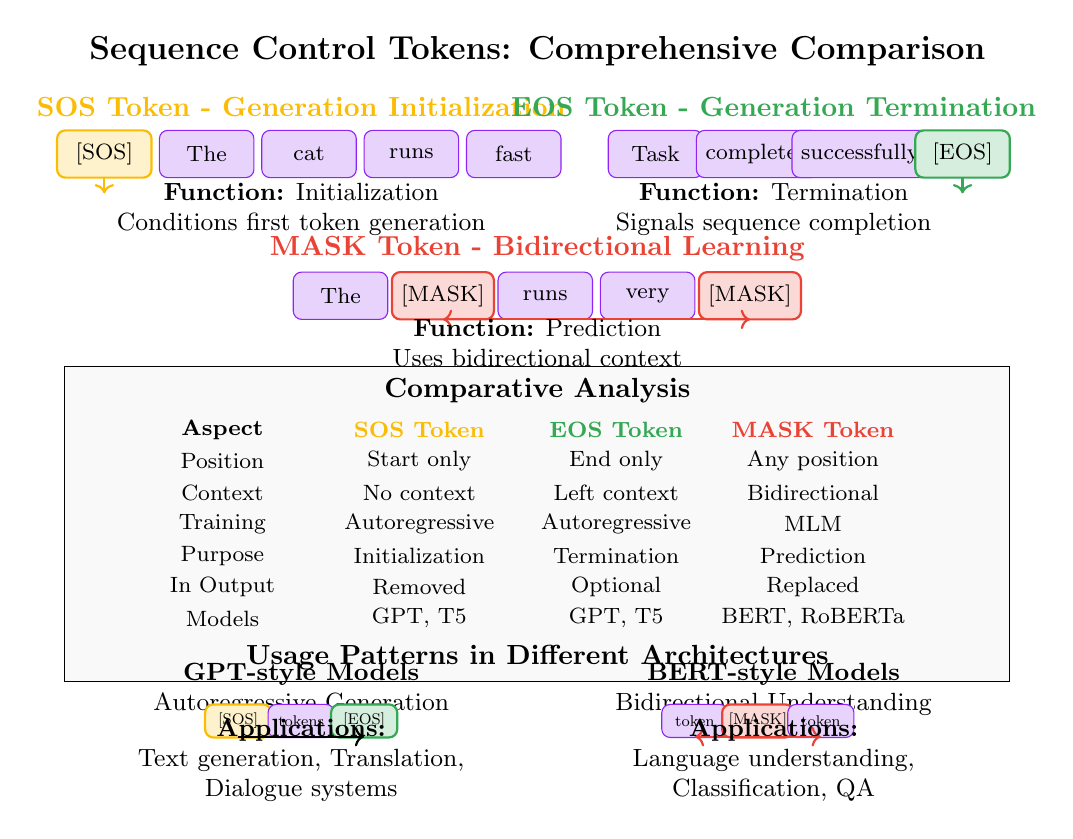
\begin{tikzpicture}[
    token/.style={rectangle, rounded corners=3pt, minimum width=1.2cm, minimum height=0.6cm, font=\footnotesize},
    sostoken/.style={token, fill=soscolor!20, draw=soscolor, thick},
    eostoken/.style={token, fill=eoscolor!20, draw=eoscolor, thick},
    masktoken/.style={token, fill=maskred!20, draw=maskred, thick},
    normaltoken/.style={token, fill=tokencolor!20, draw=tokencolor},
    label/.style={font=\small},
    title/.style={font=\large\bfseries},
    subtitle/.style={font=\normalsize\bfseries}
]

% Title
\node[title] at (6, 9.5) {Sequence Control Tokens: Comprehensive Comparison};

% SOS Token Section
\node[subtitle, soscolor] at (3, 8.8) {SOS Token - Generation Initialization};

% SOS example
\node[sostoken] at (0.5, 8.2) {[SOS]};
\node[normaltoken] at (1.8, 8.2) {The};
\node[normaltoken] at (3.1, 8.2) {cat};
\node[normaltoken] at (4.4, 8.2) {runs};
\node[normaltoken] at (5.7, 8.2) {fast};

\draw[->, thick, soscolor] (0.5, 7.9) -- (0.5, 7.7);
\node[label, align=center] at (3, 7.5) {\textbf{Function:} Initialization\\Conditions first token generation};

% EOS Token Section
\node[subtitle, eoscolor] at (9, 8.8) {EOS Token - Generation Termination};

% EOS example
\node[normaltoken] at (7.5, 8.2) {Task};
\node[normaltoken] at (8.8, 8.2) {completed};
\node[normaltoken] at (10.1, 8.2) {successfully};
\node[eostoken] at (11.4, 8.2) {[EOS]};

\draw[->, thick, eoscolor] (11.4, 7.9) -- (11.4, 7.7);
\node[label, align=center] at (9, 7.5) {\textbf{Function:} Termination\\Signals sequence completion};

% MASK Token Section
\node[subtitle, maskred] at (6, 7) {MASK Token - Bidirectional Learning};

% MASK example
\node[normaltoken] at (3.5, 6.4) {The};
\node[masktoken] at (4.8, 6.4) {[MASK]};
\node[normaltoken] at (6.1, 6.4) {runs};
\node[normaltoken] at (7.4, 6.4) {very};
\node[masktoken] at (8.7, 6.4) {[MASK]};

\draw[<->, thick, maskred] (4.8, 6.1) -- (8.7, 6.1);
\node[label, align=center] at (6, 5.8) {\textbf{Function:} Prediction\\Uses bidirectional context};

% Comparison Table
\node[rectangle, draw=black, fill=gray!5, minimum width=12cm, minimum height=4cm] at (6, 3.5) {};
\node[subtitle] at (6, 5.2) {Comparative Analysis};

% Table headers
\node[label, font=\footnotesize\bfseries] at (2, 4.7) {Aspect};
\node[label, font=\footnotesize\bfseries, soscolor] at (4.5, 4.7) {SOS Token};
\node[label, font=\footnotesize\bfseries, eoscolor] at (7, 4.7) {EOS Token};
\node[label, font=\footnotesize\bfseries, maskred] at (9.5, 4.7) {MASK Token};

% Row 1: Position
\node[label, font=\footnotesize] at (2, 4.3) {Position};
\node[label, font=\footnotesize] at (4.5, 4.3) {Start only};
\node[label, font=\footnotesize] at (7, 4.3) {End only};
\node[label, font=\footnotesize] at (9.5, 4.3) {Any position};

% Row 2: Context
\node[label, font=\footnotesize] at (2, 3.9) {Context};
\node[label, font=\footnotesize] at (4.5, 3.9) {No context};
\node[label, font=\footnotesize] at (7, 3.9) {Left context};
\node[label, font=\footnotesize] at (9.5, 3.9) {Bidirectional};

% Row 3: Training
\node[label, font=\footnotesize] at (2, 3.5) {Training};
\node[label, font=\footnotesize] at (4.5, 3.5) {Autoregressive};
\node[label, font=\footnotesize] at (7, 3.5) {Autoregressive};
\node[label, font=\footnotesize] at (9.5, 3.5) {MLM};

% Row 4: Purpose
\node[label, font=\footnotesize] at (2, 3.1) {Purpose};
\node[label, font=\footnotesize] at (4.5, 3.1) {Initialization};
\node[label, font=\footnotesize] at (7, 3.1) {Termination};
\node[label, font=\footnotesize] at (9.5, 3.1) {Prediction};

% Row 5: Output
\node[label, font=\footnotesize] at (2, 2.7) {In Output};
\node[label, font=\footnotesize] at (4.5, 2.7) {Removed};
\node[label, font=\footnotesize] at (7, 2.7) {Optional};
\node[label, font=\footnotesize] at (9.5, 2.7) {Replaced};

% Row 6: Models
\node[label, font=\footnotesize] at (2, 2.3) {Models};
\node[label, font=\footnotesize] at (4.5, 2.3) {GPT, T5};
\node[label, font=\footnotesize] at (7, 2.3) {GPT, T5};
\node[label, font=\footnotesize] at (9.5, 2.3) {BERT, RoBERTa};

% Usage patterns
\node[subtitle] at (6, 1.8) {Usage Patterns in Different Architectures};

% GPT-style (autoregressive)
\node[label, align=center] at (3, 1.4) {\textbf{GPT-style Models}\\Autoregressive Generation};
\node[sostoken, scale=0.7] at (2.2, 1.0) {[SOS]};
\node[normaltoken, scale=0.7] at (3, 1.0) {tokens};
\node[eostoken, scale=0.7] at (3.8, 1.0) {[EOS]};
\draw[->, thick] (2.2, 0.8) -- (3.8, 0.8);

% BERT-style (bidirectional)
\node[label, align=center] at (9, 1.4) {\textbf{BERT-style Models}\\Bidirectional Understanding};
\node[normaltoken, scale=0.7] at (8, 1.0) {token};
\node[masktoken, scale=0.7] at (8.8, 1.0) {[MASK]};
\node[normaltoken, scale=0.7] at (9.6, 1.0) {token};
\draw[<->, thick, maskred] (8, 0.8) -- (9.6, 0.8);

% Applications
\node[label, align=center] at (3, 0.5) {\textbf{Applications:}\\Text generation, Translation,\\Dialogue systems};

\node[label, align=center] at (9, 0.5) {\textbf{Applications:}\\Language understanding,\\Classification, QA};

\end{tikzpicture}
\end{document}